\documentclass[11pt,a4paper]{report}

% ============================================================
% PACKAGES
% ============================================================

\usepackage[utf8]{inputenc}
\usepackage[T1]{fontenc}
\usepackage[french]{babel}
\usepackage{longtable}
% Mise en page
\usepackage{geometry}
\geometry{
    top=2.5cm,
    bottom=2.5cm,
    left=2.7cm,
    right=2.7cm
}

% Images et figures
\usepackage{graphicx}
\usepackage{float}
\usepackage{caption}

% Couleurs
\usepackage{xcolor}

% Liens
\usepackage{hyperref}

% Titres
\usepackage{titlesec}

% En-têtes et pieds de page
\usepackage{fancyhdr}

% Listes
\usepackage{enumitem}

% Espacement
\usepackage{setspace}

% Tableaux
\usepackage{array}

% ============================================================
% COULEURS
% ============================================================

\definecolor{mainblue}{RGB}{31,78,121}
\definecolor{darkblue}{RGB}{20,55,90}
\definecolor{lightblue}{RGB}{235,242,249}
\definecolor{graytext}{RGB}{90,90,90}
\definecolor{lightgray}{RGB}{240,240,240}

% ============================================================
% HYPERREF
% ============================================================

\hypersetup{
    colorlinks=true,
    linkcolor=mainblue,
    urlcolor=mainblue,
    citecolor=mainblue,
    pdftitle={Documentation Technique},
    pdfauthor={Maha El Allam},
    pdfsubject={Documentation technique et fonctionnelle}
}

% ============================================================
% STYLE GENERAL
% ============================================================

\onehalfspacing

\setlength{\parindent}{0pt}
\setlength{\parskip}{0.6em}

% ============================================================
% STYLE DES CHAPITRES
% ============================================================

\titleformat{\chapter}[display]
    {\normalfont\bfseries\color{mainblue}}
    {\filleft\Large\chaptertitlename\ \thechapter}
    {0.5cm}
    {\Huge\filright}
    [\vspace{0.3cm}\titlerule]

\titlespacing*{\chapter}
    {0pt}
    {-20pt}
    {35pt}

% ============================================================
% STYLE DES SECTIONS
% ============================================================

\titleformat{\section}
    {\Large\bfseries\color{darkblue}}
    {\thesection}
    {0.8em}
    {}

\titlespacing*{\section}
    {0pt}
    {2.2em}
    {1em}

\titleformat{\subsection}
    {\large\bfseries\color{mainblue}}
    {\thesubsection}
    {0.8em}
    {}

\titlespacing*{\subsection}
    {0pt}
    {1.5em}
    {0.7em}

% ============================================================
% STYLE DES LISTES
% ============================================================

\setlist[itemize]{
    leftmargin=1.2cm,
    itemsep=0.35em,
    topsep=0.5em
}

\setlist[enumerate]{
    leftmargin=1.2cm,
    itemsep=0.5em,
    topsep=0.5em
}

% ============================================================
% STYLE DES FIGURES
% ============================================================

\captionsetup{
    font=small,
    labelfont=bf,
    labelsep=colon,
    justification=centering,
    skip=8pt
}

% ============================================================
% EN-TÊTES ET PIEDS DE PAGE
% ============================================================

\pagestyle{fancy}

\fancyhf{}

\fancyhead[L]{
    \small\color{graytext}\textit{Documentation Technique}
}

\fancyhead[R]{
    \small\color{graytext}\textit{Gestion des Allotements Hôteliers}
}

\fancyfoot[C]{
    \small\color{graytext}\thepage
}

\renewcommand{\headrulewidth}{0.4pt}
\renewcommand{\footrulewidth}{0pt}

% Style des pages de chapitre
\fancypagestyle{plain}{
    \fancyhf{}
    \fancyfoot[C]{\small\color{graytext}\thepage}
    \renewcommand{\headrulewidth}{0pt}
    \renewcommand{\footrulewidth}{0pt}
}

% ============================================================
% CONFIGURATION DU SOMMAIRE
% ============================================================

\addto\captionsfrench{
    \renewcommand{\contentsname}{Sommaire}
}

% ============================================================
% DOCUMENT
% ============================================================

\begin{document}

% ============================================================
% PAGE DE GARDE
% ============================================================

\begin{titlepage}

    \thispagestyle{empty}

    \begin{center}

        \vspace*{0.8cm}

        % Logo
        
\includegraphics[width=0.22\textwidth]{image/logo_entreprise.jpg}

        \vspace{1.5cm}

        % Nom de l'entreprise
        {\Large\bfseries Smart Holol}

        \vspace{1.8cm}

        % Ligne décorative
        {\color{mainblue}\rule{0.82\textwidth}{1.5pt}}

        \vspace{0.6cm}

        % Titre
        {\Huge\bfseries\color{darkblue}
        Documentation Technique
        }

        \vspace{0.5cm}

        {\Large\color{graytext}
        Développement et Intégration d'une Solution
        }

        \vspace{0.6cm}

        {\color{mainblue}\rule{0.82\textwidth}{1.5pt}}

        \vspace{2.2cm}

        % Cadre du document
        \fcolorbox{mainblue}{lightblue}{
            \begin{minipage}{0.72\textwidth}
                \centering
                \vspace{0.45cm}

                {\Large\bfseries\color{darkblue}
                Grille Fonctionnelle
                }

                \vspace{0.45cm}
            \end{minipage}
        }

        \vspace{2.5cm}

        % Informations
        \renewcommand{\arraystretch}{1.7}

        \begin{tabular}{>{\centering\arraybackslash}p{5.5cm}
                        >{\centering\arraybackslash}p{5.5cm}}

            \textbf{\color{darkblue}Réalisé par}
            &
            \textbf{\color{darkblue}Entreprise}
            \\[0.15cm]

            \hline

            Maha El Allam
            &
            Smart Holol

        \end{tabular}

        \vfill

        % Pied de page de la couverture
        {\color{mainblue}\rule{\textwidth}{0.6pt}}

        \vspace{0.4cm}

        {\large
        Documentation de réalisation
        }

        \vspace{0.2cm}

    \end{center}

\end{titlepage}

% ============================================================
% SOMMAIRE
% ============================================================

\cleardoublepage
\phantomsection
\vspace{0.8cm}
\tableofcontents
\cleardoublepage

% ============================================================
% CONTENU DU DOCUMENT
% ============================================================

\chapter{ALLOTEMENTS HÔTELIERS}

\section{Étape 1 : Configuration des Articles}

Pour qu'Odoo puisse gérer le stock des nuitées, les chambres ne doivent pas être créées en tant que services, mais en tant qu'articles physiques gérés en stock.

\begin{itemize}
    \item \textbf{Type d'article :} Définir le produit comme \textbf{Bien} (impératif pour que le module Inventaire puisse le suivre).
    \item \textbf{Route / Logistique :} S'assurer qu'aucune règle de réapprovisionnement automatique (MTO) ne vient interférer, car l'allotement est un stock initial fixe.
\end{itemize}


\section{Étape 2 : Configuration des Emplacements}

Pour isoler les stocks par hôtel :

\begin{enumerate}
    \item Activer le mode développeur sur Odoo.
    \item Aller dans \textbf{Inventaire > Configuration > Paramètres} et cocher \textbf{Emplacements d'inventaire multiples}.
    \item Créer un emplacement parent de type \textit{Vue} nommé \textbf{Hôtels}.
    \item Créer des emplacements enfants pour chaque hôtel (ex: \textit{Hôtels/Hôtel A}).
\end{enumerate}


\section{Étape 3 : Entrée du Stock Initial (Allotement)}

L'allotement contractuel est injecté manuellement dans le système via un ajustement d'inventaire :

\begin{itemize}
    \item Accéder à \textbf{Inventaire > Opérations > inventaire physique}.
    \item Sélectionner l'emplacement spécifique de l'hôtel (ex: \textit{Hôtels/Hôtel A}).
    \item Ajouter l'article de type chambre et renseigner la quantité contractuelle dans \textbf{Quantité comptée}.
    \item Valider l'inventaire pour initialiser le stock disponible.
\end{itemize}


\section{Étape 4 : Développement Spécifique (Blocage et Décrémentation)}

Par défaut, Odoo autorise la vente même en cas de rupture de stock. Pour un hôtel, il est indispensable de bloquer la vente si le nombre de nuitées demandées dépasse l'allotement disponible.

\textbf{Si on veut bloquer les ventes si le stock est épuisé :}

\textbf{On va au produit : onglet Vente > En rupture de stock > Décocher Continuer la vente.}

\newpage

% ============================================================
% ALERTES DISPONIBILITES
% ============================================================

\chapter{ALERTES DISPONIBILITÉS}

La mise en place des alertes de seuil pour la gestion des contingents hôteliers s'effectue entièrement à l'aide des fonctionnalités standard du module \textbf{Inventaire} d'Odoo, selon les étapes suivantes :

\section{Étape 1 : Paramétrage de l'Article Stockable}

Accéder au menu \texttt{Inventaire > Produits > Produits}.

\begin{figure}[H]
    \centering
    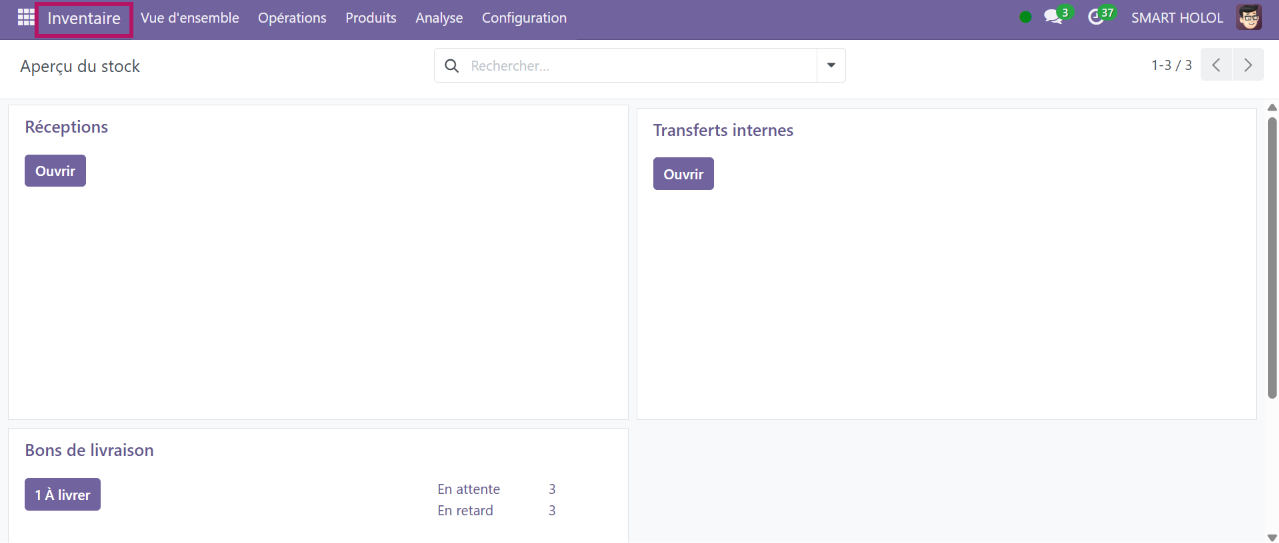
\includegraphics[width=\linewidth]{image/inventaire/inventaire8.png}
    \caption{Accès au module Inventaire}
    \label{fig:inv8}
\end{figure}

\begin{figure}[H]
    \centering
    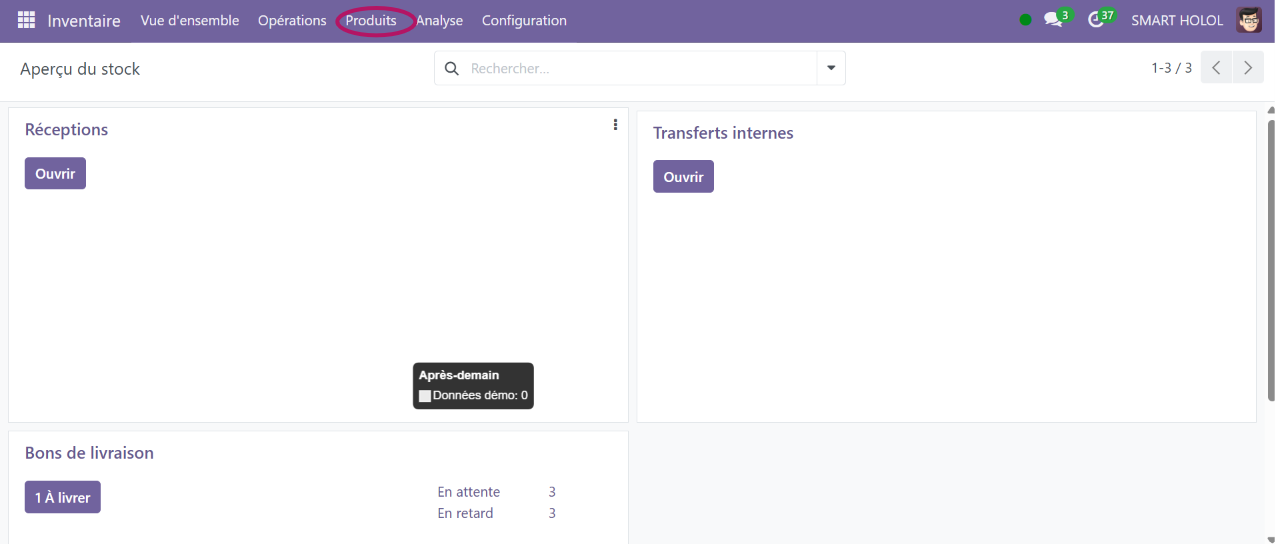
\includegraphics[width=\linewidth]{image/inventaire/inventaire9.png}
    \caption{Sélection du menu Produit}
    \label{fig:inv9}
\end{figure}

\begin{figure}[H]
    \centering
    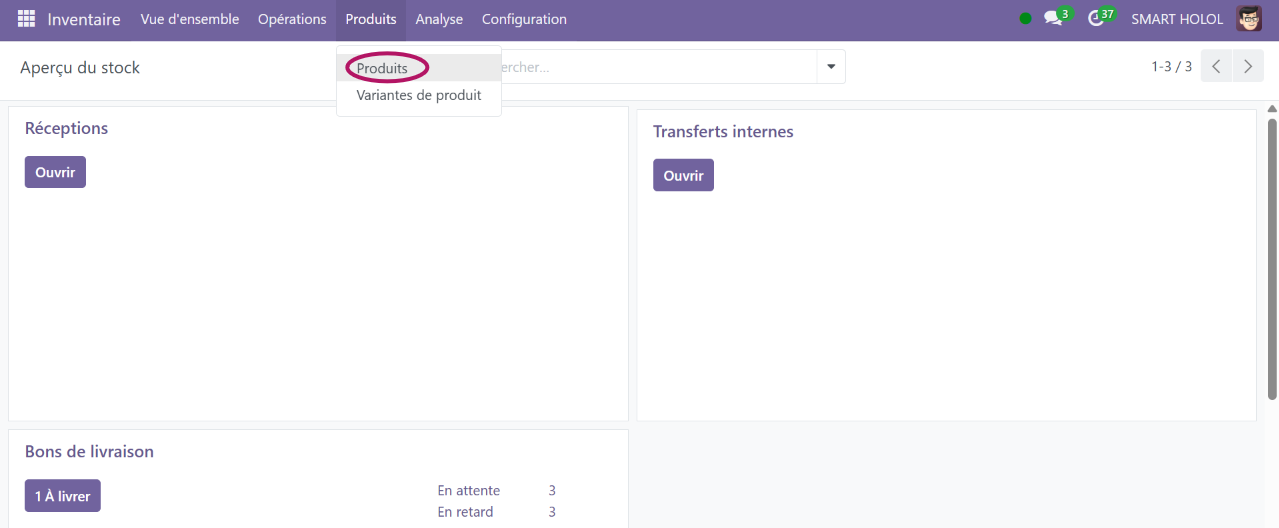
\includegraphics[width=\linewidth]{image/inventaire/inventaire10.png}
    \caption{Sélection du menu Produit}
    \label{fig:inv10}
\end{figure}

Configurer le type d'article en tant que \textbf{Article stockable (Bien)} afin de permettre le suivi des mouvements de stock et des quantités disponibles.

\begin{figure}[H]
    \centering
    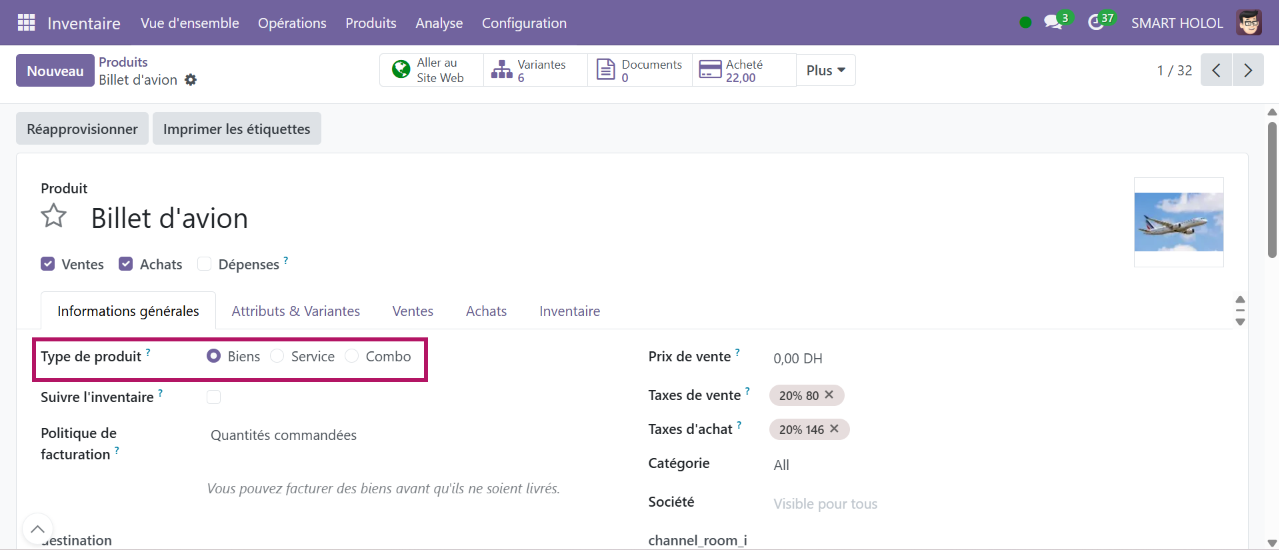
\includegraphics[width=\linewidth]{image/inventaire/inventaire11.png}
    \caption{Configuration de l'article en tant que bien stockable}
    \label{fig:inv11}
\end{figure}


\section{Étape 2 : Configuration de la Règle de Réassort}

Naviguer vers \texttt{Inventaire > Opérations > Approvisionnement > Réassort}.

\begin{figure}[H]
    \centering
    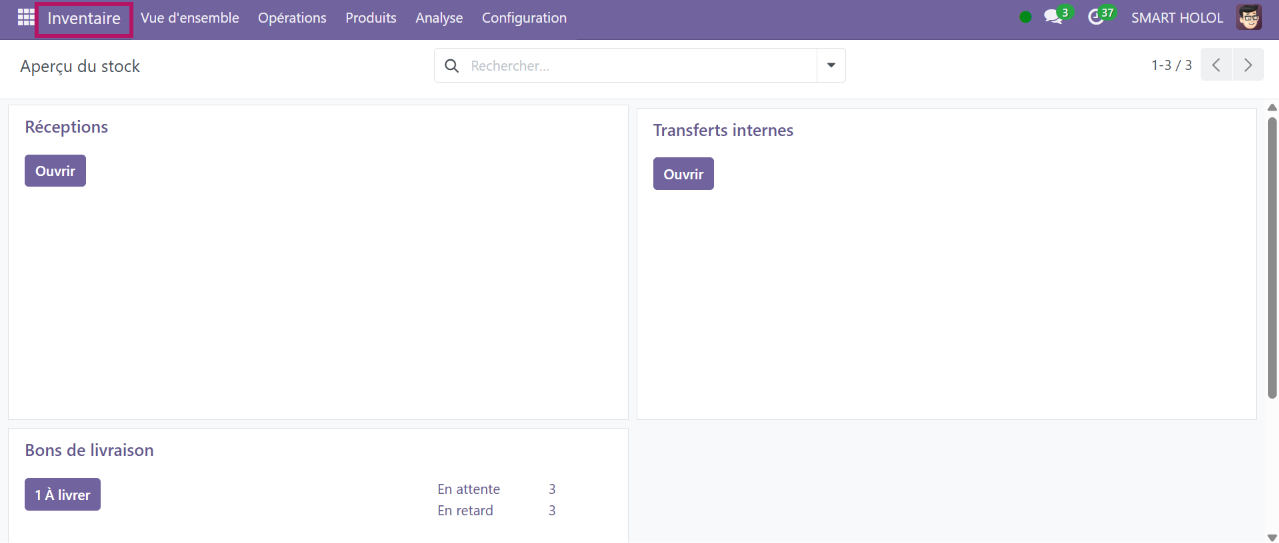
\includegraphics[width=\linewidth]{image/inventaire/inventaire8.png}
    \caption{Accès au menu de gestion du réassort}
    \label{fig:inv8_bis}
\end{figure}

\begin{figure}[H]
    \centering
    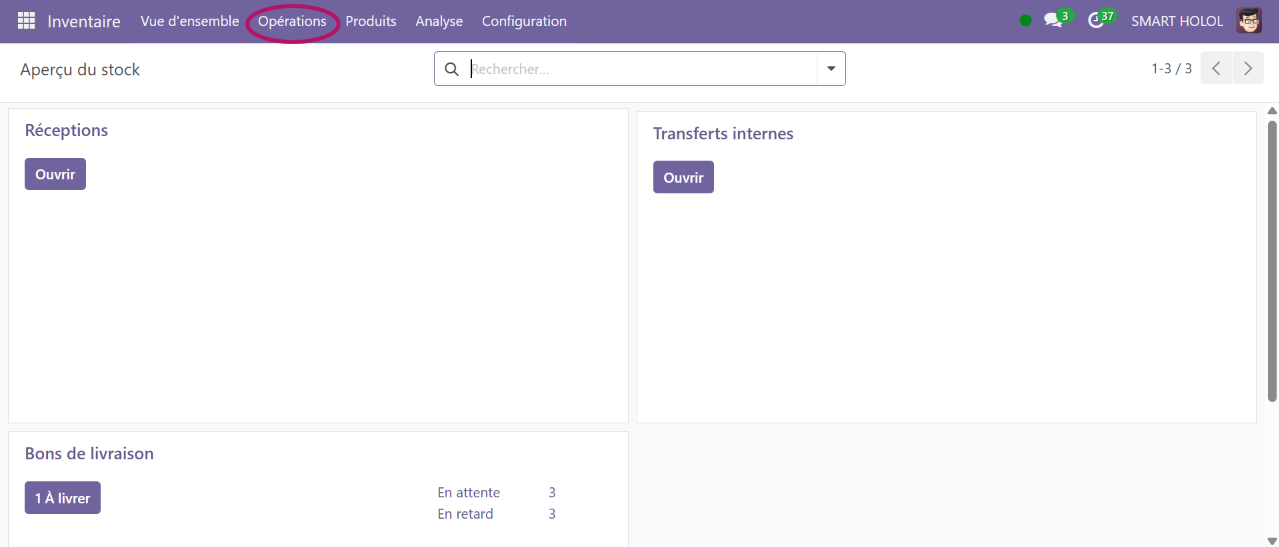
\includegraphics[width=\linewidth]{image/inventaire/inventaire12.png}
    \caption{Accès à l'interface de gestion des règles de réassort}
    \label{fig:inv12}
\end{figure}

\begin{figure}[H]
    \centering
    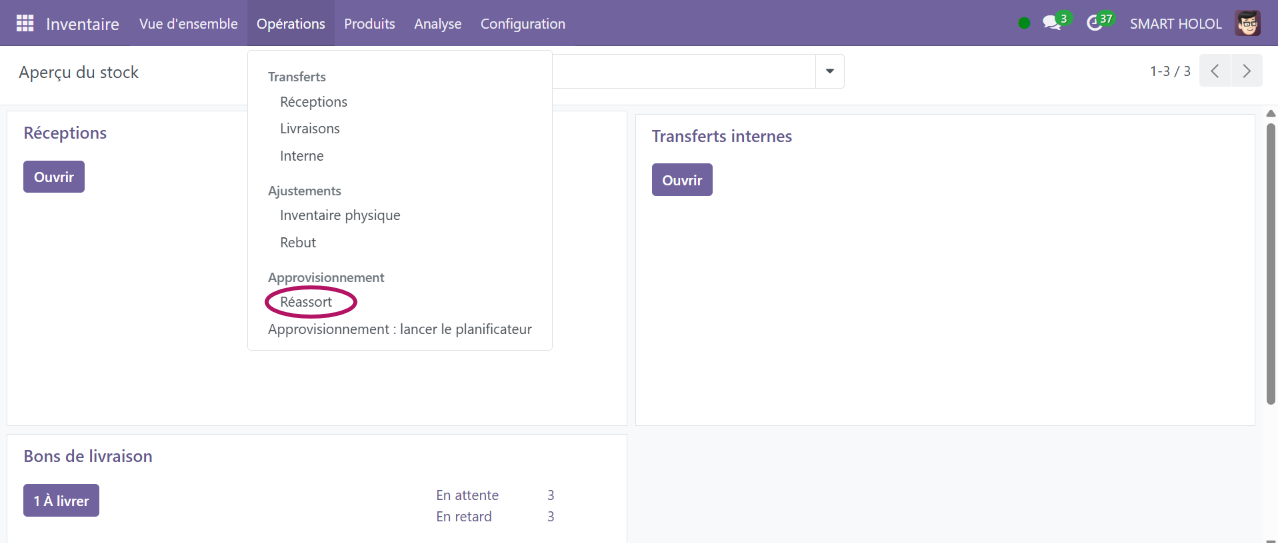
\includegraphics[width=\linewidth]{image/inventaire/inventaire13.png}
    \caption{Consultation des règles de réassort existantes}
    \label{fig:inv13}
\end{figure}

Créer une nouvelle règle en renseignant :

\begin{figure}[H]
    \centering
    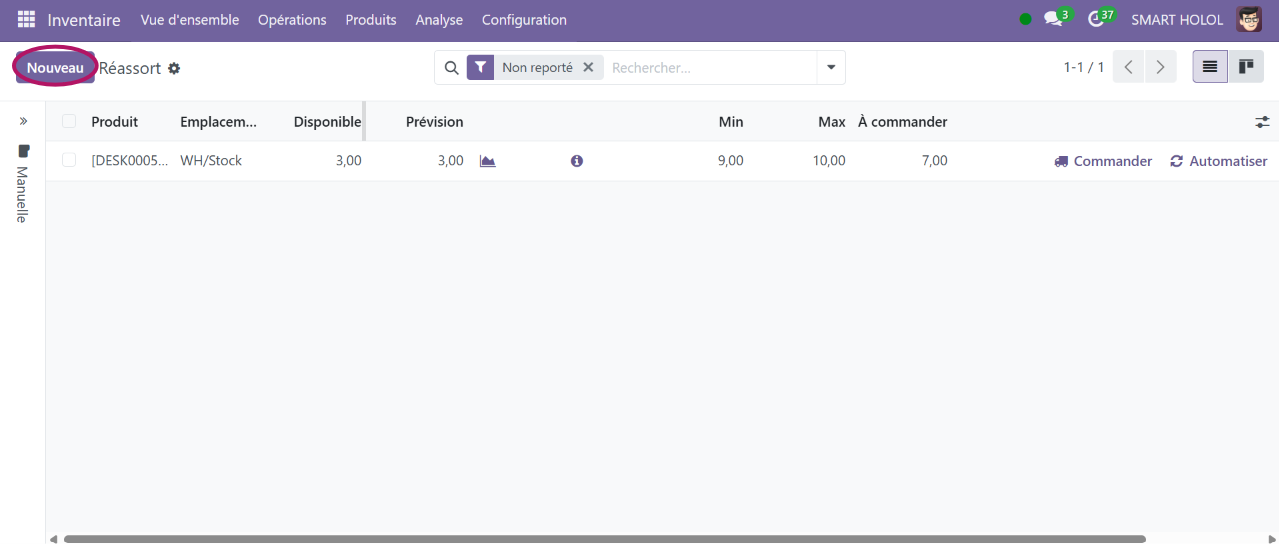
\includegraphics[width=\linewidth]{image/inventaire/inventaire14.png}
    \caption{Création et paramétrage d'une nouvelle règle de réassort}
    \label{fig:inv14}
\end{figure}

\begin{itemize}
    \item L'\textbf{Article} (ex. type de chambre).
    \item L'\textbf{Emplacement} de stockage dédié.
    \item La \textbf{Quantité minimale} (seuil critique déclenchant l'alerte).
    \item La \textbf{Quantité maximale} (allotement total contractuel).
\end{itemize}

\begin{figure}[H]
    \centering
    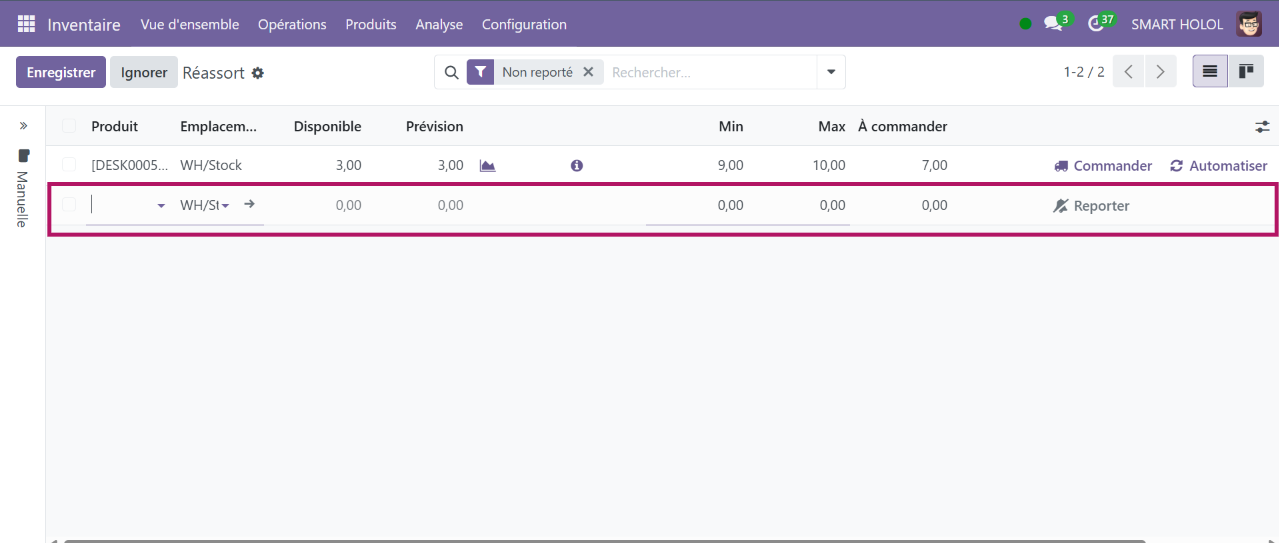
\includegraphics[width=\linewidth]{image/inventaire/inventaire15.png}
    \caption{Définition des seuils minimal et maximal du stock}
    \label{fig:inv15}
\end{figure}


\section{Étape 3 : Simulation et Déclenchement de l'Alerte}

Enregistrer une commande client (devis validé) entraînant une sortie de stock, puis valider le bon de livraison associé afin de décrémenter le stock effectif en dessous du seuil minimal.

\begin{figure}[H]
    \centering
    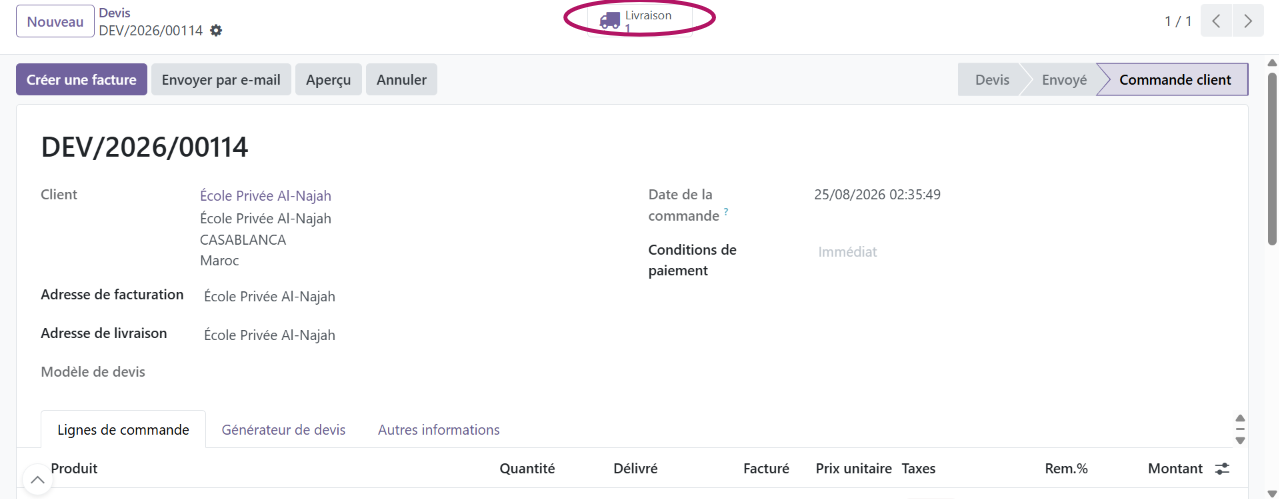
\includegraphics[width=\linewidth]{image/inventaire/inventaire16.png}
    \caption{Validation du bon de livraison entraînant la diminution du stock}
    \label{fig:inv16}
\end{figure}

Une alerte en vert \og Pas disponible \fg{} s'affiche alors, ainsi qu'une alerte supplémentaire lors de la validation de l'opération.

\begin{figure}[H]
    \centering
    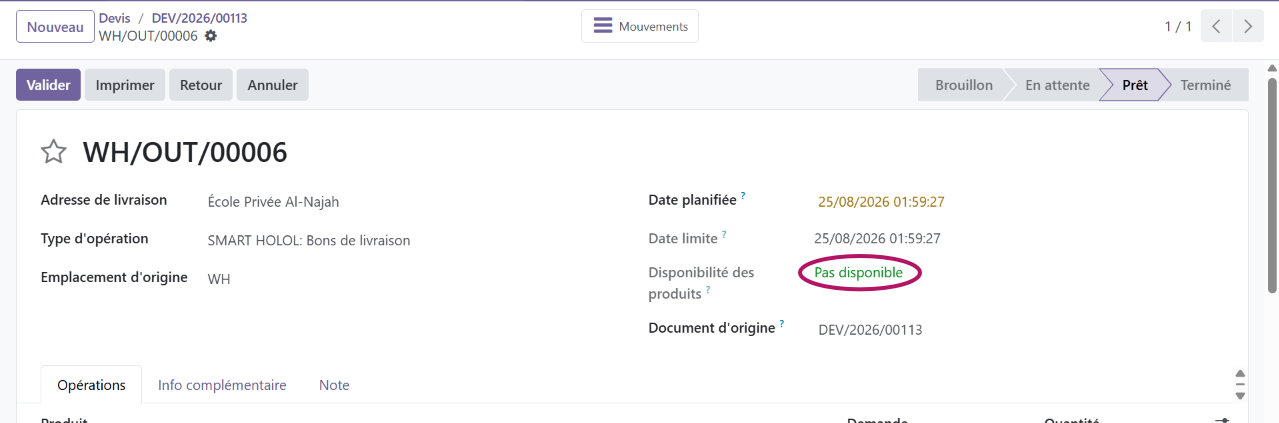
\includegraphics[width=\linewidth]{image/inventaire/inventaire17.png}
    \caption{Affichage de l'alerte de disponibilité du produit}
    \label{fig:inv17}
\end{figure}

\begin{figure}[H]
    \centering
    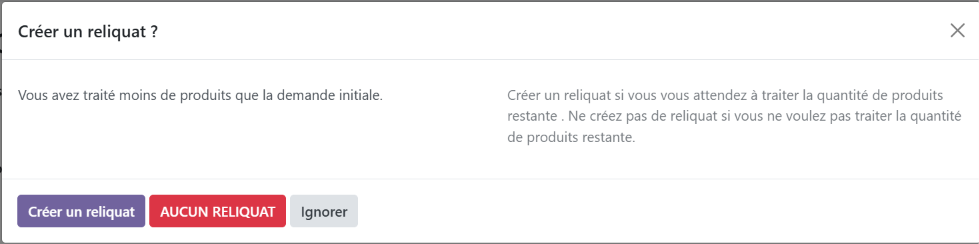
\includegraphics[width=\linewidth]{image/inventaire/inventaire18.png}
    \caption{Notification affichée lors de la validation de la livraison}
    \label{fig:inv18}
\end{figure}

\newpage

% ============================================================
% CONTRATS HOTELIERS
% ============================================================

\chapter{CONTRATS HÔTELIERS}

\section{Étape 1 : Configuration des Hôtels et Archivage des Contrats}

Chaque hôtel partenaire est enregistré en tant que fournisseur :

Rendez-vous dans le module \textbf{Achats > Commandes > Fournisseurs}.

\begin{figure}[H]
    \centering
    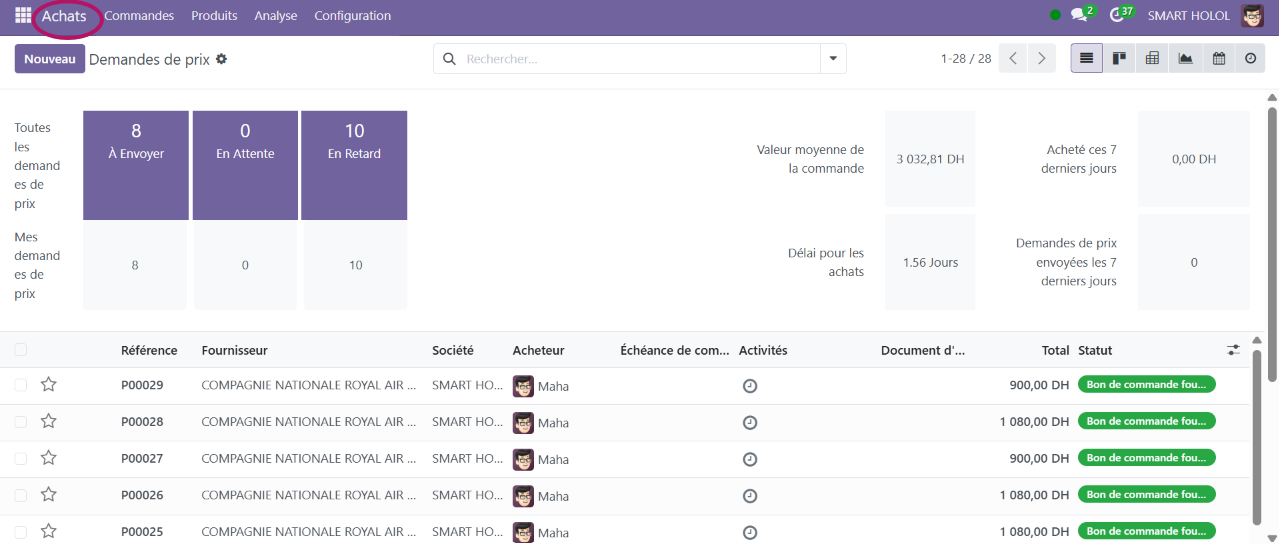
\includegraphics[width=\linewidth]{image/contrats_hoteliers/fournisseur1.png}
    \caption{Accès au module Achats}
    \label{fig:fourn1}
\end{figure}

\begin{figure}[H]
    \centering
    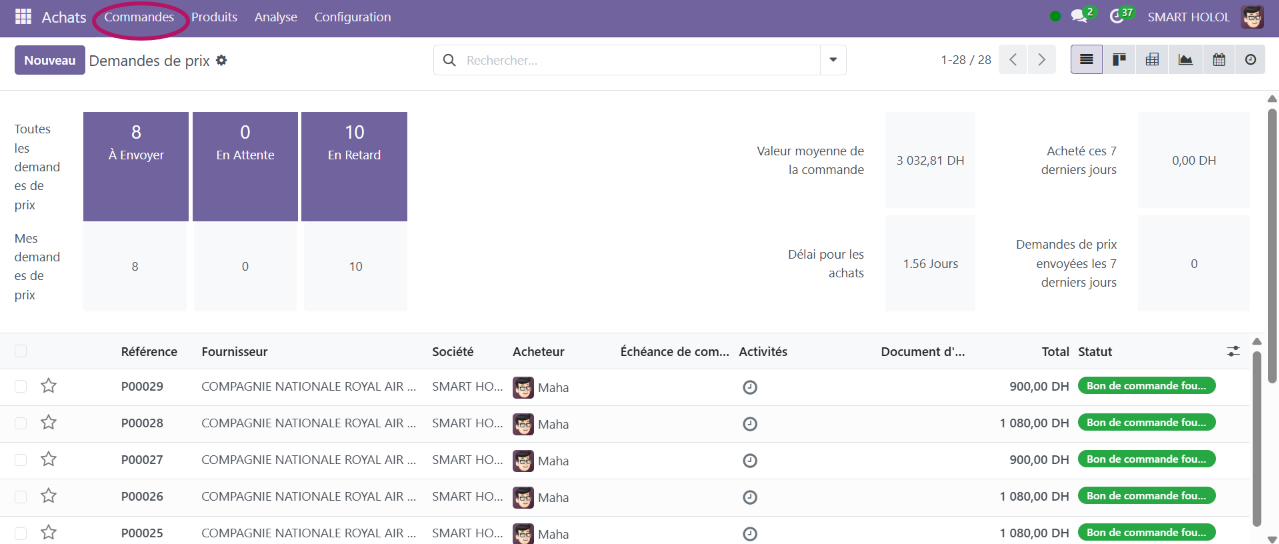
\includegraphics[width=\linewidth]{image/contrats_hoteliers/fournisseur2.png}
    \caption{Accès au menu commandes}
    \label{fig:fourn2}
\end{figure}

\begin{figure}[H]
    \centering
    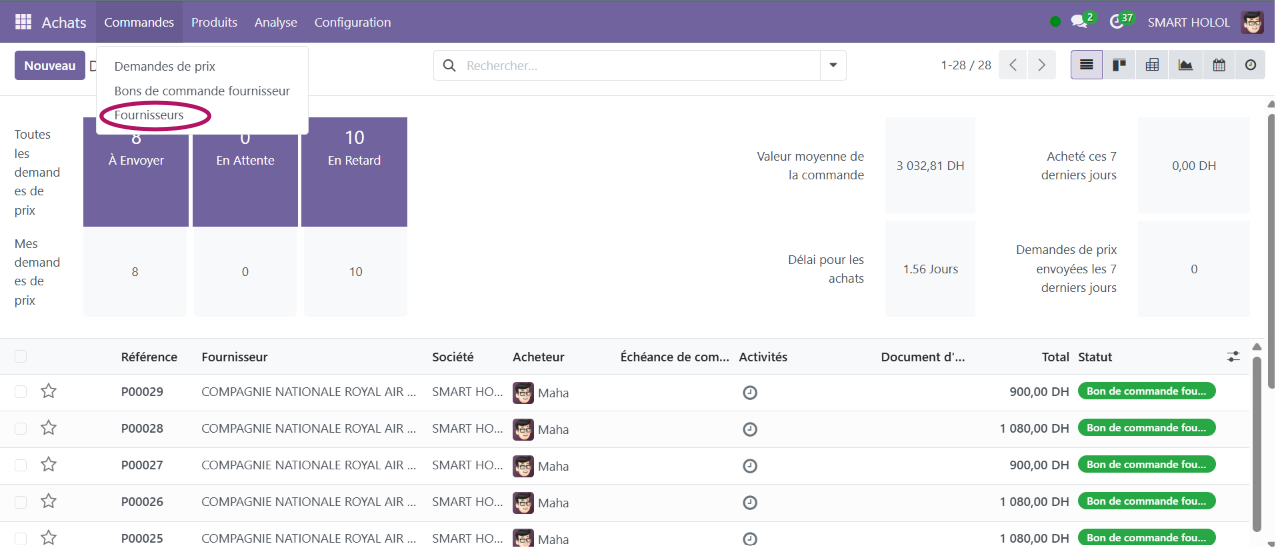
\includegraphics[width=\linewidth]{image/contrats_hoteliers/fournisseur3.png}
    \caption{Accès au menu fournisseur}
    \label{fig:fourn3}
\end{figure}

Créez ou ouvrez la fiche de l'hôtel. La présence du bouton intelligent \textit{Achats} en haut à droite confirme son rôle de fournisseur.

\begin{figure}[H]
    \centering
    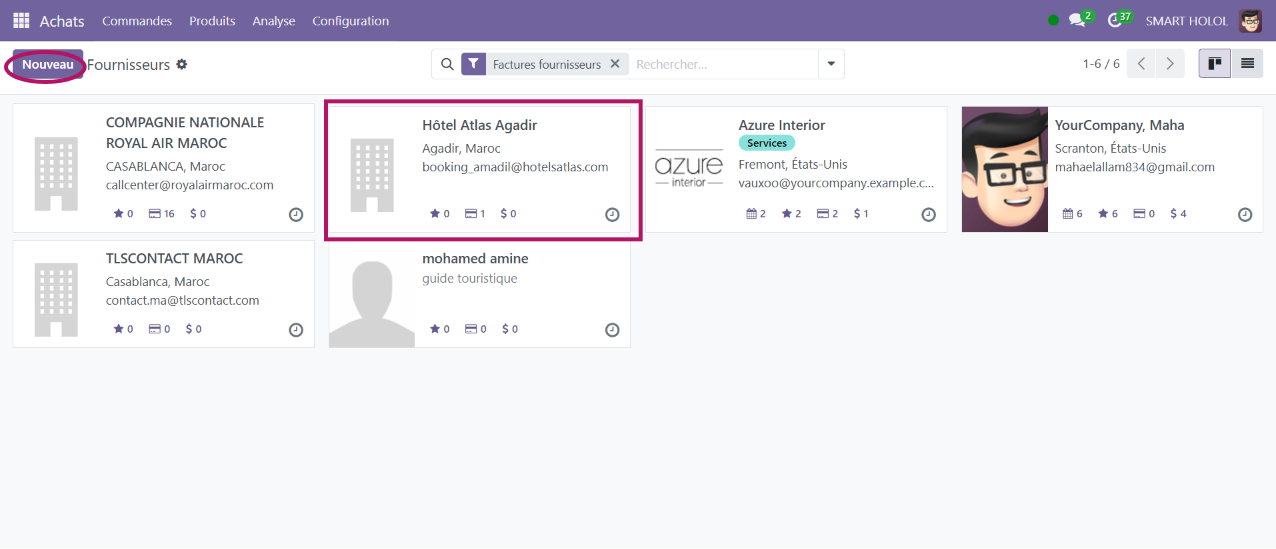
\includegraphics[width=\linewidth]{image/contrats_hoteliers/fournisseur4.png}
    \caption{Page fournisseur}
    \label{fig:fourn4}
\end{figure}

\textbf{Sécurité et Traçabilité :} Dans le coin inférieur gauche de la fiche contact, utilisez le widget des pièces jointes (icône trombone) pour téléverser le contrat hôtelier signé au format PDF ainsi que les grilles tarifaires papier.

\begin{figure}[H]
    \centering
    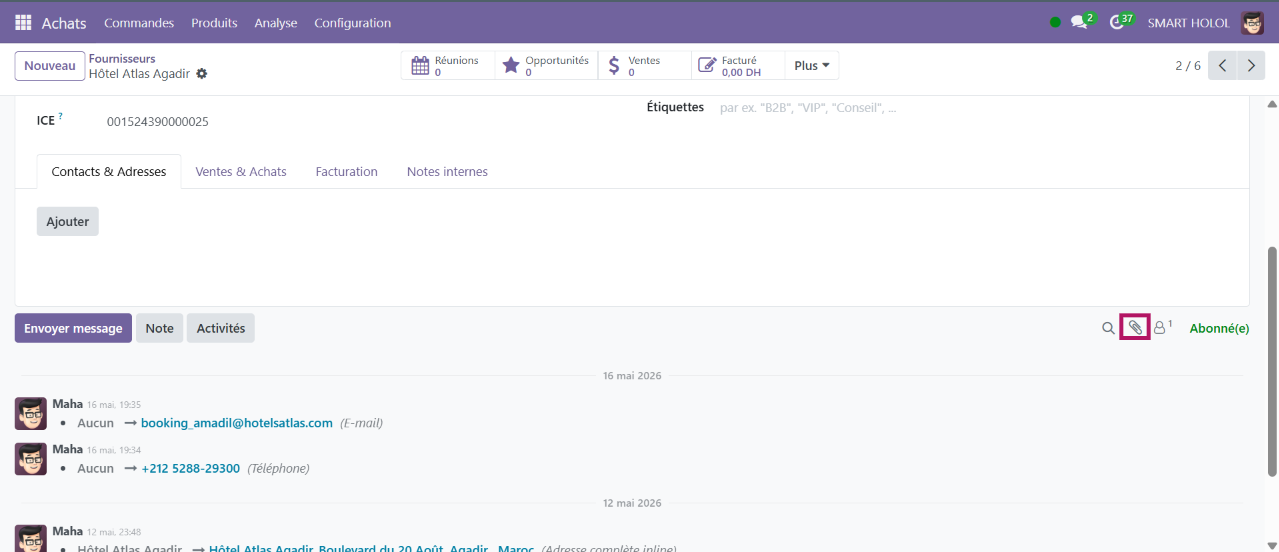
\includegraphics[width=\linewidth]{image/contrats_hoteliers/fournisseur5.png}
    \caption{Pièces jointes et traçabilité sur la fiche fournisseur}
    \label{fig:fourn5}
\end{figure}


\section{Étape 2 : Création des Articles (Types de Chambres et Prestations)}

Pour chaque typologie de chambre ou service :

\begin{enumerate}
    \item Allez dans \textbf{Achats > Produits > Produits}.
    \item Créez un article (ex. : \textit{Chambre Double Standard}) avec le type \textbf{Service}.
    \item Renseignez le prix de vente public applicable aux clients.
\end{enumerate}


\section{Étape 3 : Gestion des Saisons et Grilles Tarifaires}

Pour lier les prix d'achat négociés par période (Haute, Moyenne, Basse saison) :

\begin{enumerate}
    \item Ouvrez la fiche de l'article (ex. : \textit{Chambre Double Standard}) et accédez à l'onglet \textbf{Achats}.
    \item Dans la section \textit{Fournisseurs}, ajoutez une ligne pour chaque hôtel et chaque saison :
    \begin{itemize}
        \item \textbf{Ligne Haute Saison :} Sélection de l'hôtel, prix d'achat fort, et définition de la période de validité (si les champs de dates sont actifs) ou création d'un article dédié par saison (ex. : \textit{Chambre Double - Haute Saison}).
        \item \textbf{Ligne Basse Saison :} Définition du tarif réduit pour la période creuse.
    \end{itemize}
\end{enumerate}


\section{Étape 4 : Application dans les Devis Clients}

\begin{enumerate}
    \item Allez dans le module \textbf{Ventes > Devis > Créer}.
    \item Sélectionnez le client et ajoutez l'article hôtelier correspondant.
    \item Odoo va automatiquement récupérer le coût d'achat associé via le fournisseur, permettant un calcul instantané de la marge commerciale et une centralisation fluide des contrats.
\end{enumerate}

\chapter{ÉTAT D'AVANCEMENT DU PROJET}

La grille fonctionnelle suivante présente l'état d'avancement des différents modules et intégrations développés dans le cadre du projet.

\begingroup
\setlength{\LTpre}{10pt}
\setlength{\LTpost}{10pt}
\begin{longtable}{|p{3cm}|p{8.5cm}|c|}
    \hline
    \textbf{Module / Fonctionnalité} & \textbf{Observations et État d'Avancement} & \textbf{Statut} \\ \hline
    \endhead

    \hline \multicolumn{3}{r}{\textit{(Suite sur la page suivante)}} \\ \hline
    \endfoot

    \hline
    \endlastfoot

    % Partie Bleue / Connexions & Stock & Contrats
    \textbf{API Sabre} & Implémenté via une API minimaliste ne retournant pas des résultats complets. & En cours \\ \hline
    
    \textbf{API Hotelbeds} & Intégration et communication fonctionnelles. & Fait \\ \hline
    
    \textbf{Autres APIs (Amadeus, Galileo, RateHawk, WebBeds)} & Absence de clés d'accès pour établir la communication. & En attente \\ \hline
    
    \textbf{Agrégateur Tarifaire} & Nécessite les retours des différentes APIs pour effectuer la comparaison. & En attente \\ \hline
    
    \textbf{Webhooks \& Sync Temps Réel} & Mise en place et synchronisation opérationnelles. & Fait \\ \hline
    
    \textbf{Gestion de Stock} & Fonctionnel, à l'exception du tableau de bord de stock non disponible sur la version gratuite. & Partiel \\ \hline
    
    \textbf{Contrats Hôteliers} & Centralisation et gestion des contrats intégrées. & Fait \\ \hline
    
    % Partie Blanche / Modules Odoo additionnels
    \textbf{CRM} & Capture automatique des demandes de devis, qualification des préférences et planification des activités. & Fait \\ \hline
    
    \textbf{Ventes} & Configuration des devis détaillés multi-prestations, gestion des acomptes progressifs et commandes clients. & Fait \\ \hline
    
    \textbf{Facturation} & Création des factures et application des règles de gestion spécifiques (régime de TVA/marge). & Fait \\ \hline
    
    \textbf{Achats} & Centralisation de la base des prestataires (hôtels, transporteurs) et émission des bons de commande. & Fait \\ \hline
    
    \textbf{Dossiers de Voyage} & Création automatique de dossiers logistiques (projets/tâches) et suivi des check-lists opérationnelles. & Fait \\ \hline
    
    \textbf{Site Web} & Vitrine moderne des packages de voyage, réservation directe en ligne et portail client sécurisé. & Fait \\ \hline
    
    \textbf{Ressources Humaines} & Planification des plannings des guides accompagnateurs et gestion des notes de frais terrains. & Fait \\ \hline

    \textbf{Inventaire \& Emplacements} & Création des articles stockables et définition des emplacements multiples par hôtel. & Fait \\ \hline

\end{longtable}
\endgroup
% ============================================================
% FIN DU DOCUMENT
% ============================================================

\end{document}